\biohead{Kathleen Munday}{}{ }

Katheen Munday was born at 8 Shalston Villas, Surbiton at 3:30 pm on 5th November 1882\cite{JHMtree, KMbirthCert, JHMbible} and christened on 18 July 1883 in Surbiton. She was the second daughter of \bioref{John_Hill_Munday} and \bioref{Catherine_Aldridge}. She had four siblings: \bioref{Nora_Katie_Munday}, \bioref{Mildred_Mary_Munday}, \bioref{Ralph_Munday} and \bioref{Margery_Munday}.
They lived at The Mendips, Surbiton, Surrey.  She was educated at Cheltenham Ladies College, but like most middle class women of her generation did not receive a higher education, nor did she seek employment after finishing school. She was a very accomplished wood carver and artist and received a medal for her fine work (see photographs). She met \bioref{James_Denton_Barker} when she was on holiday at Ilkley and they married just before the outbreak of the first World War on 4th April 1914 at the Wandsworth Registry Office.\cite{KathleenJamesWeddingIndex} The notice in \emph{The Times} read:

\begin{quotation}
The Marriage of Miss Kathleen Munday, second daughter of Mr. and Mrs. J.\ H.\ Munday, of Cedar Lodge, St.\ Johns Road, Putney, with Mr. James Denton Barker, of Liverpool, took place very quietly in London on the 4th inst. The bride was married in her travelling dress of blue serge, with a black tagal hat trimmed with a pale blue ostrich feather and a pink rose. Mr and Mrs J. Denton Barker left immediately after the ceremony for the Yorkshire moors and the Lake District, where the honeymoon is being spent, prior to taking up their residence in Liverpool. A reception was held on the previous day by the bride's mother, which was attended by a number of guests, when the many very handsome presents were on view.
\end{quotation}

Early the following year their first son, \bioref{Bertram_Mead_Denton_Barker}, was born,
followed a year and a half later by \bioref{Ralph_Munday_Denton-Barker},
and then \bioref{Virginia_Kathleen_Denton_Barker}.

For most of their married life, James and Kathleen lived in Birkenhead (at 'Beechwood', Mt. Pleasant) and in later years in Harpenden, Hertfordshire. After James' death, she moved to Leeds to live near her daughter Virginia, and she died on 17 September 1963. The probate announcement read: ``\textsc{Barker, Kathleen} of Laurel Bank, Templar lane, Stanks, Leeds widow died 17 September 1963 at The Grand Infirmary, Leeds. Probate Wakefield 14 November to Virginia Kathleen Denton Grebenik (wife of Eugene Grebenik) and D. McCandlish Bell solicitor. \pounds29,594~8s.''

\begin{figure}
\centering
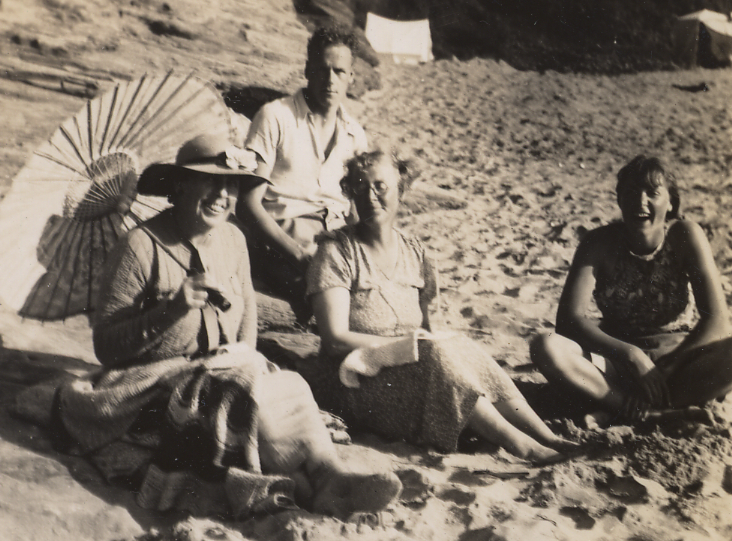
\includegraphics{photos/Barker_family_c1939}
\caption{\bioref{Nora_Katie_Munday}, \bioref{Ralph_Munday}, \bioref{Kathleen_Munday}, and \bioref{Virginia_Kathleen_Denton_Barker} in about 1939.}
\end{figure}

\begin{figure}
\centering
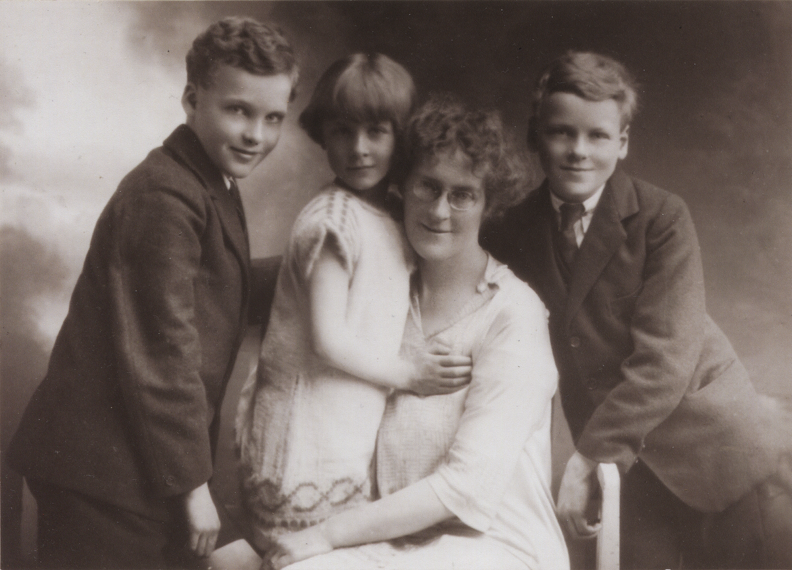
\includegraphics{photos/Mead_Virginia_Kathleen_and_Ralph.png}
\caption{Mead, Virginia, Kathleen, and Ralph.}
\end{figure}
